\documentclass[english,12pt, titlepage]{article}
\usepackage{graphicx} % Required for inserting images
\usepackage[margin=1in]{geometry}
\usepackage{amsmath}
\usepackage{blindtext}
\usepackage{mathtools}
\usepackage{fullpage}
\usepackage{array}
%\usepackage[T1]{fontenc}
%\usepackage{babel}
%\title{\textbf{Stochastic Differential Equation and Applications}}
\begin{center}
	{ \bfseries Evaluating Optimal Techniques for Data Fitting and Forecasting: Identifying the Best Approach for Accurate Predictions  }\vspace{3 \baselineskip}
	
	{\Large  Project Report}\vspace{2 \baselineskip}
	
	{\Large \underline{ Submitted by:}\vspace{5mm} \\ \textbf{Abdul Wahab}\vspace{2mm} \\ \textbf{Idris Oduola} \\ \textbf{Abdul Rahman}\vspace{2mm} \\ \textbf{Notik}} \vspace{3.5\baselineskip}
	
	{\Large Instructor:  \textbf{Dr. Selim Belhaiza}} \vspace{0.5\baselineskip}
	
	{\Large }
	\vspace{0.5\baselineskip}
	
	{\Large \bfseries Department of Mathematics \\ and Statistics  } \vspace{3\baselineskip}
	
	\begin{figure}[h]
		\centering
		\includegraphics[width=0.4\linewidth]{logo}
		\label{fig:logo}
	\end{figure}
	
	{\Large King Fahd University of Petroleum and Minerals Dhahran, Saudi Arabia \bfseries}
	\vspace{3.5\baselineskip}
\end{center}
\newpage
%\author{Abdul Wahab & Ayesha Siddiqua\\{Course Instructor:} Dr. Boubakar Smii}
%\textbf{King Fahad University of Petroleum and Minerals, Dhahran, Saudi Arabia}
%\title{\huge\textbf{Stochastic Differential Equation and it's Application}}
%\author{ Abdul Wahab, Ayesha Siddiqua}
%\textbf{Course Instructor:}
%\textbf{Dr. Boubakar Smii}
%\date{16 November 2023}









\begin{document}
	
	\newpage
	
	\tableofcontents
	
	\newpage
	
	
	
	
	
	
	\section{Introduction}
	In numerous domains, from energy management and finance to healthcare and engineering, the precision of data fitting and forecasting is paramount. Developing models that accurately predict future trends or fit historical data necessitates the selection of techniques tailored to the specific characteristics of the dataset. This research focuses on assessing optimal techniques for data fitting and forecasting through a combination of statistical methods and machine learning algorithms, including Exploratory Data Analysis (EDA), Variance-Covariance Analysis, Linear Regression, Singular Value Decomposition (SVD), Time Series Analysis, and Neural Networks with varying activation functions, neurons, and layers.\\
	
	Exploratory Data Analysis (EDA) offers foundational insights into the dataset's structure, enabling the identification of patterns, anomalies, and relationships between variables. It represents the initial step in ensuring data readiness for advanced modeling techniques \cite{jt}.\\
	
	Variance-Covariance Analysis measures relationships and dependencies among variables, facilitating the selection of critical predictors and minimizing data redundancy \cite{jw}.\\
	
	Traditional Linear Regression serves as a baseline model, providing interpretability and efficiency for datasets exhibiting linear relationships. However, for datasets requiring dimensionality reduction or optimization of computational efficiency, Singular Value Decomposition (SVD) is utilized to identify dominant patterns while reducing noise \cite{gvl}.\\
	
	Time Series Analysis is particularly beneficial for datasets with sequential dependencies, capturing trends and seasonality to forecast future values \cite{box}. For more complex and non-linear relationships, Neural Networks offer a robust framework, especially when employing different activation functions (e.g., ReLU, sigmoid, tanh) and experimenting with varying numbers of neurons and layers to enhance predictive accuracy \cite{gf}.\\
	
	This study evaluates each technique individually and compares hybrid models, such as integrating time series models with neural networks and autoregressive methods. The objective is to identify the best-performing approaches in terms of accuracy, scalability, and computational efficiency, contributing to the ongoing exploration of data-driven decision-making strategies in real-world applications.
	
	
	\newpage
	\section{Methodology}
	This study employs a systematic and multi-faceted approach to evaluate optimal techniques for data fitting and forecasting. Below is the detailed step-by-step methodology:
	\subsection{Exploratory Data Analysis (EDA)}
	
	\begin{itemize}
		\item \textbf{Objective:} Understand the dataset's structure and identify patterns, outliers, and relationships.
		\item \textbf{Data Cleaning:}
		
		Remove missing values or impute them using statistical methods.
		Detect and handle outliers using boxplots and interquartile range (IQR) techniques.
		\item \textbf{	Visualization:}
		
		Generate visualizations like histograms, scatter plots, and correlation matrices to observe relationships between variables.
		Use pair plots to detect multicollinearity or clustering tendencies.
		\item 	\textbf{Feature Engineering:}
		
		Transform categorical variables into numeric forms (e.g., one-hot encoding).
		Normalize or standardize features to ensure consistency across scales.
	\end{itemize}
	\subsection{ Variance-Covariance Analysis}
	\begin{itemize}
		\item 	\textbf{Objective:} Analyze interdependencies between variables to identify significant predictors.
		\item \textbf{Covariance Matrix:}
		
		Compute the covariance matrix to measure how variables vary with respect to one another.
		
		\item \textbf{Principal Variables: }Identify features with high variance and strong relationships, indicating their importance in the model.
		\item \textbf{	Dimensionality Reduction:}
		
		Use the covariance matrix to prepare data for SVD or reduce redundant features before applying complex models.
	\end{itemize}
	
	\subsection{Baseline Model with Linear Regression}
	\begin{itemize}
		\item \textbf{Objective:} Develop a simple and interpretable model as a benchmark.
		\item \textbf{Model Training:}
		
		Use the selected predictors to fit a linear regression model.
		Split the dataset into training and testing sets (e.g., 80/20 split).
		\item 	\textbf{Evaluation:}
		
		Measure model performance using Mean Squared Error (MSE), R-squared, and residual analysis.
		
		\item 	\textbf{Insights:} Identify any limitations of linear regression, such as an inability to capture non-linear relationships.
		
	\end{itemize}
	
	\subsection{Singular Value Decomposition (SVD)}
	\begin{itemize}
		\item 	\textbf{Objective:} Perform dimensionality reduction to enhance computational efficiency and robustness.
		%		\item 	\textbf{Matrix Decomposition:} 	Apply SVD to decompose the dataset matrix $A$ into $U \sum V^{T}$, where $U$ and $V$ are orthogonal matrices, and $\sum$ contain singular values.  
		\item \textbf{Matrix Decomposition:} Apply SVD to decompose the dataset matrix $A$ into $U \Sigma V^{T}$, where $U$ and $V$ are orthogonal matrices, and $\Sigma$ contains the singular values.
		
		\item 
		\textbf{	Feature Selection:}
		
		Retain components corresponding to the largest singular values, representing dominant patterns.
		\item \textbf{Model Refinement:}
		
		Reconstruct the data using the selected components and retrain predictive models to evaluate performance.
	\end{itemize}
	
	\subsection{Time Series Analysis}
	\begin{itemize}
		\item \textbf{Objective:} Capture sequential dependencies, trends, and seasonality for forecasting purposes.
		\item 
		\textbf{	Data Preparation:}
		
		Format the dataset for time series analysis by setting a temporal index.
		
		\item \textbf{Modeling:}
		
		Fit models such as ARIMA or Exponential Smoothing for forecasting.
		
		\item \textbf{Diagnostics:}
		
		Evaluate residuals to confirm the absence of autocorrelation or unmodeled seasonality.
	\end{itemize}
	
	
	\subsection{Neural Networks with Hyperparameter Tuning}
	\begin{itemize}
		\item \textbf{	Objective: }Capture non-linear dependencies using flexible neural network architectures.
		\item 	
		\textbf{Network Design:}
		
		Experiment with different activation functions (ReLU, sigmoid, tanh) to study their impact on learning.
		Vary the number of neurons and hidden layers to optimize model performance.
		\item 	\textbf{Training:}
		
		Use backpropagation with gradient descent to minimize loss functions like MSE.
		Regularize the model using techniques such as dropout or L2 regularization to prevent overfitting.
		\item \textbf{	Validation:}
		
		Evaluate the model on a validation dataset to monitor performance and fine-tune hyperparameters.
	\end{itemize}
	
	
	
	\subsection{Comparative Analysis of Models}
	
	\begin{itemize}
		\item \textbf{ Objective:} Identify the best-performing model.
		\item 	\textbf{Performance Metrics:}
		
		Compare models based on MSE, Mean Absolute Error (MAE), R-squared, and computation time.
		\item \textbf{	Hybrid Models:}
		
		Combine time series predictions with neural network outputs to enhance forecasting accuracy.
		\item \textbf{	Error Analysis:}
		
		Analyze residual errors to identify model strengths and weaknesses.
	\end{itemize}
	
	\subsection{Conclusion and Interpretation}
	\begin{itemize}
		\item  \textbf{	Objective: }Summarize findings and suggest the most suitable approach.
		\item 	\textbf{Final Selection:}
		Determine the best model based on performance metrics and the application context.
		\item 	\textbf{Applications:}
		Discuss the practical implications of the findings in real-world scenarios, such as energy consumption forecasting or financial trend prediction.
	\end{itemize}
	
	
	
	\newpage
	\section{Implementation}
	\subsection{Exploratory Data Analysis (EDA)}
	Exploratory Data Analysis (EDA) is a critical first step in understanding and preparing a dataset for analysis and modeling. The primary goal of EDA is to uncover underlying patterns, detect anomalies, and summarize the dataset’s main characteristics through both statistical and graphical methods. This process begins with data cleaning, where missing values are addressed by either removing the affected rows or imputing them using mean, median, or predictive methods. Additionally, outliers are identified using techniques such as boxplots or the interquartile range (IQR) method, as they may distort model predictions if left untreated.
	
	Following data cleaning, visualization techniques are applied to gain intuitive insights. Scatter plots and pair plots are used to observe relationships between variables, while histograms and density plots help analyze data distributions. Correlation matrices are particularly useful for identifying multicollinearity among features, as they highlight variable dependencies through correlation coefficients. These insights guide the selection of meaningful predictors for the model.
	
	In cases where the dataset contains categorical variables, feature engineering becomes necessary to encode them into numeric formats using techniques like one-hot encoding. This ensures compatibility with mathematical models. Additionally, normalizing or standardizing the numerical features is performed to maintain consistency in scales and prevent certain features from dominating the model due to larger ranges.
	
	Through these steps, EDA provides a comprehensive understanding of the dataset, enabling informed decisions about feature selection, transformation, and readiness for advanced modeling. By laying a strong foundation, EDA minimizes potential biases and enhances the effectiveness of subsequent analytical techniques.	
	
	\subsubsection{Descriptive Statistics of Data}

	\begin{figure}[!ht]
		\centering
		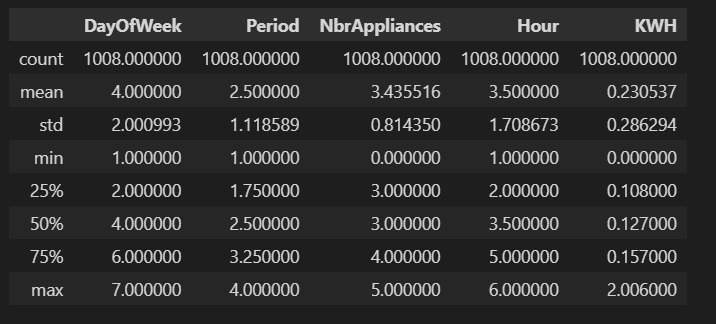
\includegraphics[width=0.6\linewidth]{fig7.jpeg}
		\caption{Table shows the Statistics of Data.}\label{fig81}
	\end{figure}
	
		This Fig.$\ref{fig81}$ summarizes key statistics for a dataset on energy usage and related variables. The DayOfWeek column represents days numerically (1 for Monday to 7 for Sunday), with an average value of 4, indicating data mostly from midweek, and variability spanning all days. The Period column likely divides time into four blocks, with most data centered around periods 2 and 3. The NbrAppliances column shows an average of 3 to 4 appliances being used at any given time, ranging from 0 to a maximum of 5. The Hour column, measured on a 6-hour scale, suggests mid-to-late operational hours with an average of 3.5. The KWH column, representing energy consumption, has a low average of 0.23 kWh, with most usage below 0.16 kWh, but peaks reaching 2.006 kWh, indicating occasional high-consumption events. Overall, the dataset captures moderate energy usage with variability in time, day, and appliance activity.
	
	\begin{figure}[!ht]
		\centering
		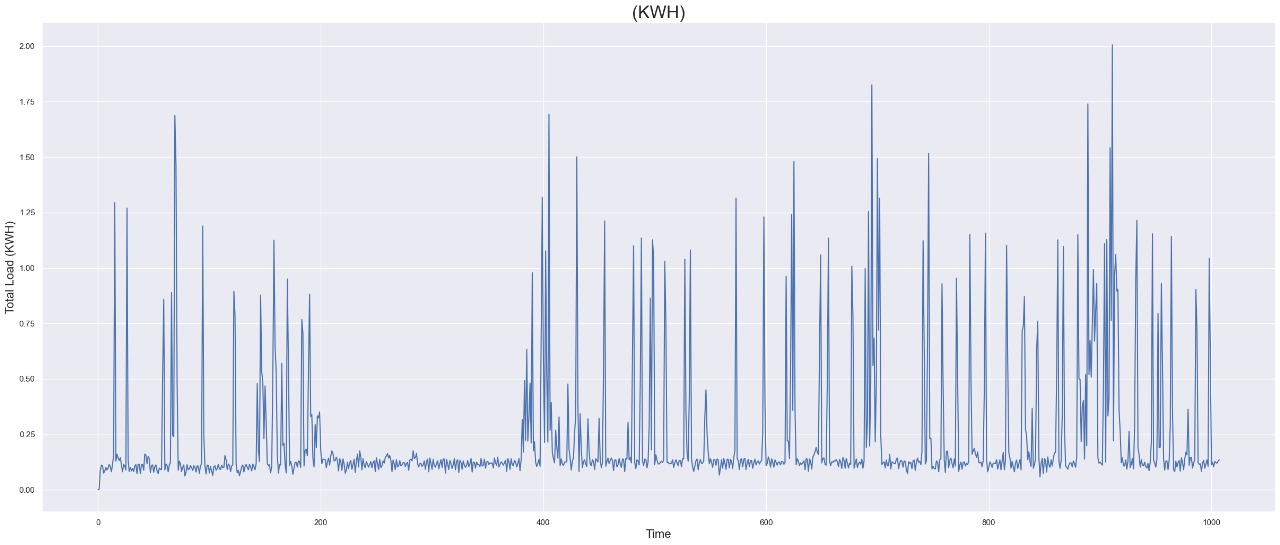
\includegraphics[width=0.6\linewidth]{fig35.jpeg}
		\caption{figure shows the KWH values over the time.}\label{fig80}
	\end{figure}
	
	This Fig.$\ref{fig80}$ illustrates the total energy load over time, measured in kilowatt-hours (kWh). The x-axis represents time, while the y-axis shows the energy load, ranging from 0 to 2 kWh. The line graph displays fluctuating energy usage with a baseline of relatively low consumption interspersed with sharp spikes, indicating short periods of high energy demand. These spikes occur irregularly, suggesting intermittent use of energy-intensive devices or appliances. Overall, the data reveals a pattern of consistent low-level consumption punctuated by sudden peaks, possibly reflecting varying operational cycles or user activities over time.
	
	
	\subsubsection{Null Value Check}
	
	Checking for null values in the dataset for all the variables shown in Fig. $\ref{fig1}$.
	The dataset had no null values. Hence no treating or imputation was required.
	
	\begin{figure}[!ht]
		\centering
		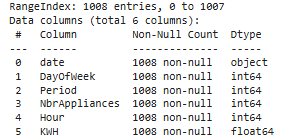
\includegraphics[width=0.6\linewidth]{tb1.png}
		\caption{Table shows the Null value Information of Data.}\label{fig1}
	\end{figure} 
	
	The table provides a summary of a dataset with 1008 rows and 6 columns, detailing the structure, data types, and completeness of the data. The date column contains information about the dates of observations and has no missing values, but it is stored as an object type, which may need to be converted into a datetime format for time-based analysis. The DayOfWeek column represents the day of the week as integers (e.g., Monday = 1) and is also complete with no missing values. Similarly, the Period column identifies specific periods within a day, potentially denoting morning, afternoon, or evening, encoded as integers. The NbrAppliances column indicates the number of appliances in use during the observation period, while the Hour column specifies the hour of the day in a 24-hour format. Both columns are complete and stored as integers. Lastly, the KWH column represents the energy consumption in kilowatt-hours (KWH), which serves as the dependent variable in the dataset and is stored as a floating-point number.
	
	The dataset is complete, with no missing values in any column, making it ready for analysis. However, preprocessing steps such as converting the date column to a proper datetime format, normalizing numerical values, or encoding categorical variables may be necessary. The clean structure and the inclusion of relevant features like day, hour, and number of appliances suggest that the dataset is well-suited for tasks like time-series analysis, regression, and predictive modeling aimed at forecasting energy consumption.
	
	\subsubsection{Target Variable}
	
	KWH are the target variable in our dataset. The variable we are attempting to estimate or predict using data from other variables in the dataset is the target variable in machine learning. It goes by the names dependent variable, the response variable, and the outcome variable.
	The KWH variable gives us the energy consumption of a household which depends upon the number of Appliances.
	
	\begin{figure}[!ht]
		\centering
		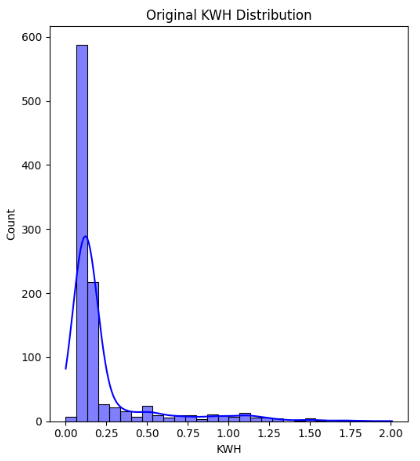
\includegraphics[width=0.5\linewidth]{fig1.png}
		\label{fig2}
	\end{figure}  
	
	The figure represents the original distribution of energy consumption (KWH) in the dataset. The histogram displays the frequency of KWH values, while the superimposed line represents the kernel density estimation (KDE), providing a smooth visualization of the data's probability density. From the plot, it is evident that the KWH distribution is highly skewed towards smaller values, with most data points concentrated near 0. This skewness indicates that the data is not normally distributed, which may pose challenges for statistical analysis and modeling techniques that assume normality. \\
	
	We will try to make the data more normally distributed, by using two common techniques, which are as following:
	
	\subsubsection{Box-Cox Transformation}
	\begin{itemize}
		\item This transformation adjusts the skewness of the data using a power transformation. The Box-Cox transformation is defined as:\\
		
		\centering
		$
		y' =
		\begin{cases} 
			\frac{y^\lambda - 1}{\lambda}, & \text{if } \lambda \neq 0 \\
			\log(y), & \text{if } \lambda = 0
		\end{cases}
		$
		
		\item Here, $\lambda$ is a parameter determined through optimization to minimize skewness.
		\item The Box-Cox transformation works only for strictly positive data. If there are zeros or negative values, a small constant can be added to the data before applying the transformation.
	\end{itemize}
	
	\begin{figure}[!ht]
		\centering
		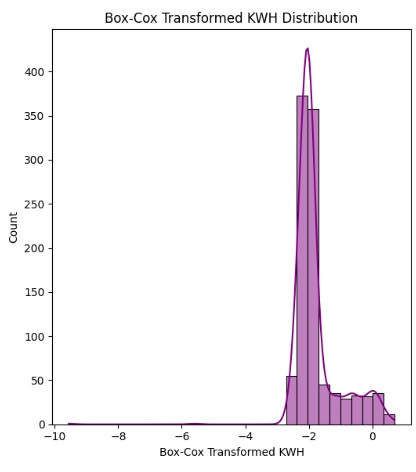
\includegraphics[width=0.5\linewidth]{fig2.jpg}
		\label{fig3}
	\end{figure}  
	This figure shows a Box-Cox transformed distribution of KWH (Kilowatt Hour) data. The histogram with a density curve overlay reveals a roughly bell-shaped but slightly right-skewed distribution. The x-axis represents the Box-Cox transformed KWH values, ranging from approximately -10 to 2, with most data concentrated between -2 and 0. The y-axis shows the count of observations, reaching a peak of around 400 counts. The highest frequency occurs near -2 on the transformed scale, creating a prominent peak. There is a noticeable right tail extending into positive values, with several smaller peaks between 0 and 2. The Box-Cox transformation was likely applied to normalize the original KWH data, though the result still shows some departure from perfect normality. The purple shading and clean presentation make the distribution pattern easily visible.
	
	The distribution in the figure is not perfectly normal due to its slight right skewness and the presence of a long tail extending into positive values. This indicates that there are some extreme values or outliers in the data that affect the overall shape of the distribution, preventing it from achieving a symmetrical bell curve characteristic of a normal distribution. Additionally, the Box-Cox transformation, while helpful in normalizing data, may not completely eliminate skewness if the original data has significant deviations from normality.
	
	Now, we will try another transformation, which is log transformation. We expecting that, this transformation will convert our data into the normal distribution as we discuss in the Box-cox transformation there is a potential outliers. That possess our data not look like normal. If the log transformation will not convert our data to the normal then we will do the outliers detection by using different methods. 
	
	\subsubsection{Log Transformation}
	\begin{itemize}
		\item This simpler approach involves taking the natural logarithm of the KWH values:
		\begin{equation*}
			y' = \log(y + c)
		\end{equation*}
		
		
		$c$ is a small constant added to ensure that all values are positive.
		
		\item The log transformation is effective in compressing large values and spreading out small values, reducing skewness.
	\end{itemize}
	
	
	\begin{figure}[!ht]
		\centering
		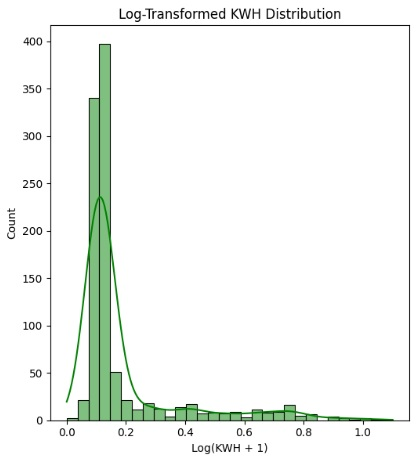
\includegraphics[width=0.5\linewidth]{fig3.jpg}
		\label{fig4}
	\end{figure}  
	The figure depicts the log-transformed distribution of the energy consumption data KWH using the log transformation 
	KWH values. The histogram indicates that the log transformation has reduced the right-skewness of the data compared to its original form. However, the distribution still deviates significantly from a normal distribution, as evident from the elongated right tail and the peak's sharpness. This suggests that the log transformation, while helpful in reducing skewness, is insufficient to normalize the data entirely.
	
	The lack of normality could arise from intrinsic properties of the data, such as heteroscedasticity or the presence of outliers. Additionally, energy consumption patterns often follow non-Gaussian distributions due to external influences such as irregular appliance usage, temporal factors (time of day or seasonality), or non-linear interactions among independent variables.
	
	\subsubsection{Outliers Detection}
	
	We can see that the both transformation do not work to make KWH normal, this is the clear indication that some values are outliers that disturb the distribution of KWH. Now, we will do the analysis of the outliers by using different method for detecting the outliers. 
	
	\begin{figure}[!ht]
		\centering
		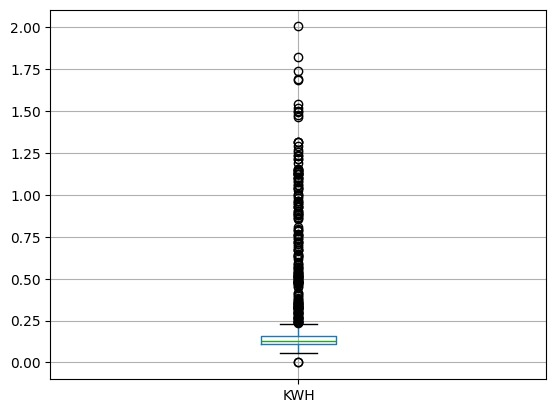
\includegraphics[width=0.6\linewidth]{fig4.jpeg}
		\caption{figures shows the position of outliers.}\label{fig5}
	\end{figure}
	
	The box plot provides a detailed visual representation of energy consumption data (KWH). The interquartile range (IQR), which lies between the first quartile (Q1) and the third quartile (Q3), represents the middle 50 percent of the data, indicating where most values are concentrated. A horizontal line within the box marks the median, showcasing the central tendency of the dataset. Whiskers extend to the smallest and largest values within 1.5 times the IQR, while any data points lying beyond this range are identified as outliers and shown as individual circles. The distribution reveals that the majority of the data points are clustered around the lower range, near 0.25 KWH, with several outliers stretching up to 2.0 KWH, suggesting a long-tailed, positively skewed distribution. This skewness reflects the presence of occasional high energy consumption instances, which deviate significantly from the majority. The presence of outliers highlights variability in the data and may result from irregular appliance usage or other exceptional circumstances. These outliers can have a substantial impact on statistical analyses and machine learning models, necessitating careful consideration during data preprocessing and modeling to ensure accurate predictions and insights.
	
	
	\begin{figure}[!ht]
		\centering
		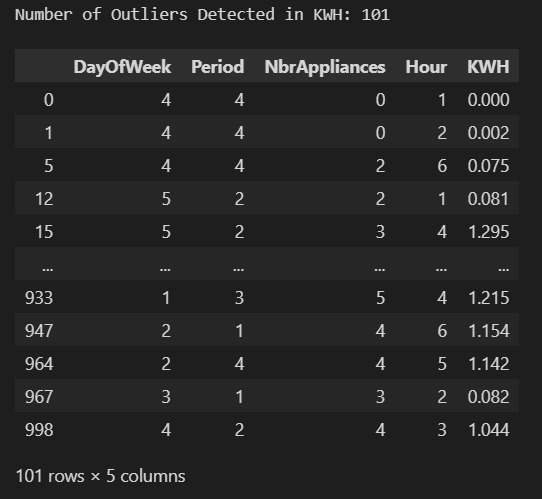
\includegraphics[width=0.5\linewidth]{fig5.jpeg}
		\caption{Table shows the number of outliers.}\label{fig6}
	\end{figure}
	
	Using the percentile, we see that the outliers is 101 which create the problem during prediction and forecasting. We remove these outliers by using percentile method can be seen in Fig. $\ref{fig6}$. 
	
	
	\begin{figure}[!ht]
		\centering
		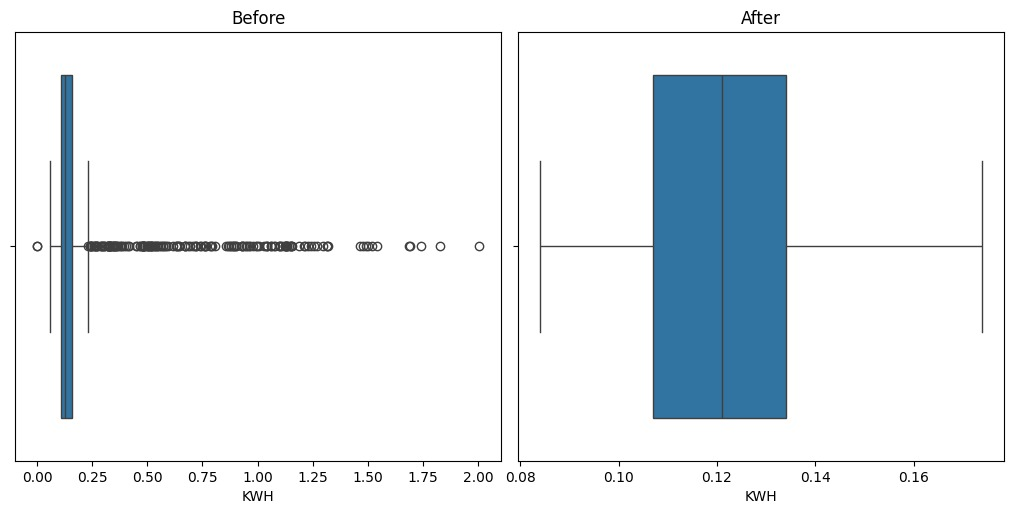
\includegraphics[width=0.7\linewidth]{fig6.jpeg}
		\caption{figure shows the big amount of outliers.}\label{fig7}
	\end{figure}
	
	Before Shape: (1008, 5)
	After Shape: (731, 5)\\
	Now, we can see that we loose a big amount of data that is why we will not use such kind of transformation. It is almost 27.5 percent of the data that this method indicates as an outliers but we do not want to loose even a single observation of our data. So, this method will not work. We will try different methods to work on outliers.\\
	
	We use the DBSCAN but again lose a big amount of data so we prefer to restrict the data as it is.    
	%%%%%%%%%%%%%%%%%%%%%%%%%%%%%%%%%%%%%%%%%%%%%%%%%%%%%%%%%%%%%%%%%%%%%%%%%%%%%%%%%%%%
	%%%%%%%%%%%%%%%%%%%%%%%%%%%%%%%%%%%%%%%%%%%%%%%%%%%%%%%%%%%%%%%%%%%%%%%%%%%%%%%%%%%%
	%%%%%%%%%%%%%%%%%%%%%%%%%%%%%%%%%%%%%%%%%%%%%%%%%%%%%%%%%%%%%%%%%%%%%%%%%%%%%%%%%%%%
	
	
	\subsection{Variance Co-Variance Method}
	
	\begin{figure}[!ht]
		\centering
		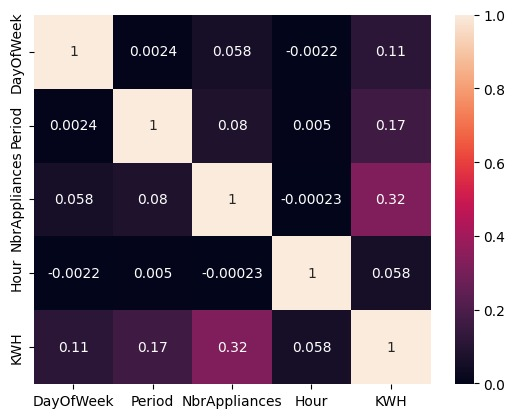
\includegraphics[width=0.6\linewidth]{fig8.jpg}
		\caption{Tables shows the correlation.}\label{fig9}
	\end{figure}
	
	The correlation matrix reveals several key relationships between the variables shown in Fig.$\ref{fig9}$. In the context of our data, when we see the correlation we observe a strong positive correlation exists between the number of appliances and energy consumption (KWH), suggesting that as more appliances are used, energy consumption increases significantly. A moderate positive correlation between period and hour indicates that certain time periods are associated with specific hours. Interestingly, a weak negative correlation is observed between the day of the week and the number of appliances, hinting at potential variations in appliance usage across different days. While these correlations provide valuable insights, it's crucial to remember that correlation does not imply causation.
	
	\subsubsection{Variance Inflation Factor}
	Now, we will also check the VIF ( Variance Inflation Factor)
	The Variance Inflation Factor (VIF) is a statistical measure used to detect multicollinearity in multiple linear regression models. It quantifies how much the variance of an estimated regression coefficient is inflated due to the correlation with other predictor variables in the model. A high VIF indicates that a predictor variable is highly correlated with other variables, leading to instability in the regression coefficients and less reliable estimates.
	
	Mathematically, the VIF for a predictor variable $X_{i}$
	is calculated as:
	
	\begin{equation*}
		VIF(X_{i}) = \frac{1}{1-R_{i}^{2}}
	\end{equation*}
	where $R_{i}$ 
	is the coefficient of determination (R-squared) from a regression of  $X_{i}$ on all other predictor variables. If $VIF(X_{i})>0$, it suggests high multicollinearity, and the variable $X_{i}$ might need to be removed or combined with other variables.
	
	
	
	The VIF is useful for diagnosing and addressing issues in models where multicollinearity can distort results, making it difficult to assess the individual effect of predictors on the dependent variable. Reducing high VIF values by removing or transforming variables can lead to more stable and interpretable regression models.
	
	
	
	\begin{figure}[!ht]
		\centering
		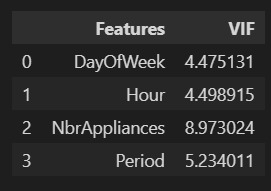
\includegraphics[width=0.35\linewidth]{fig9.jpg}
		\label{fig10}
	\end{figure}
	
	The table displays the Variance Inflation Factors (VIFs) for four features in the dataset: DayOfWeek, Hour, NbrAppliances, and Period. The VIF values for DayOfWeek and Hour are 4.48 and 4.50, respectively, indicating moderate correlation with other predictor variables. NbrAppliances has a VIF of 8.97, which suggests a higher degree of multicollinearity and may require closer attention to ensure the stability of the regression model. Period has a VIF of 5.23, also reflecting a moderate correlation with other predictors. Typically, a VIF above 5 or 10 signals potential issues with multicollinearity, and it may be necessary to reconsider the inclusion of highly correlated variables to improve the model's reliability and interpretability. These VIF values highlight the importance of assessing multicollinearity when building a regression model to ensure accurate parameter estimates.
	
	Now, we will apply the multiple linear regression model for the prediction of energy consumption but as we know data does not follow normal distribution. We expect that this model will not give good prediction. 
	
	\subsection{Multiple Linear Regression }
	
	Multiple Linear Regression (MLR) is a statistical technique used to model the relationship between one dependent variable and two or more independent variables. The goal of MLR is to find the best-fitting linear equation that predicts the value of the dependent variable based on the values of the independent variables. The model assumes that there is a linear relationship between the independent variables and the dependent variable, which in our case model can be expressed as:
	
	\begin{equation*}
		KWH = \beta_{0} + \beta_{1}(\text{DayOfWeek})  + \beta_{2}(\text{Period})  + \beta_{3}(\text{NbrAppliances}) +\beta_{4}( \text{Hour}) + \epsilon
	\end{equation*}
	where KWH is the dependent variable and others are independent variables, $\beta_{0}$ is the intercept, $\beta_{1}, \beta_{2}, \beta_{3}, \beta_{4}$ are the coefficient and $\epsilon$ is the error term. 
	
	
	\begin{figure}[!ht]
		\centering
		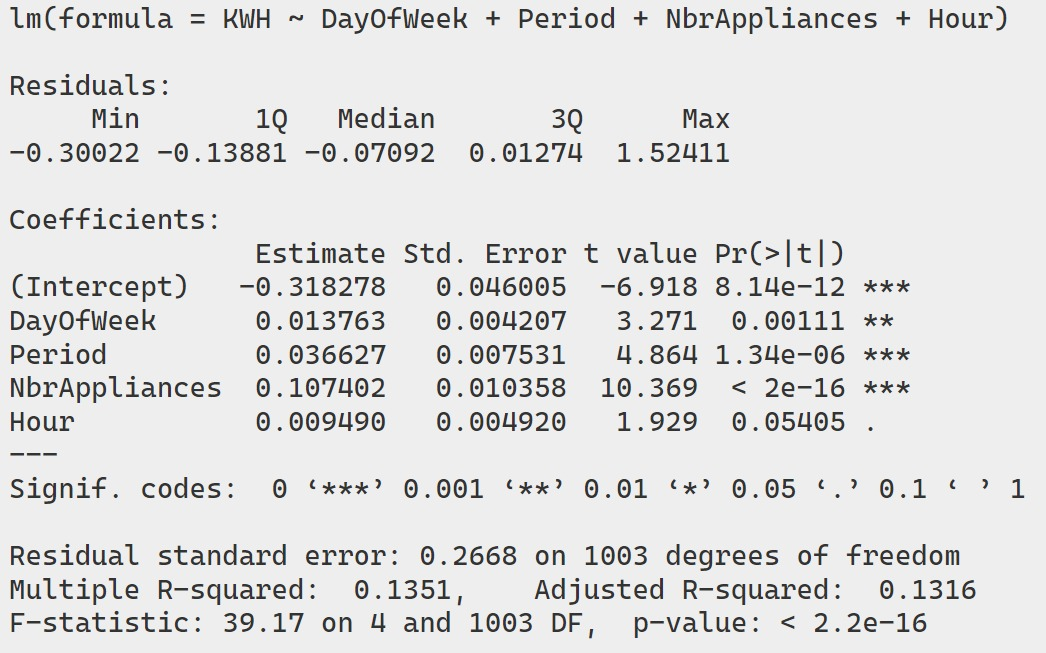
\includegraphics[width=0.55\linewidth]{fig10.jpeg}
		\label{fig11}
	\end{figure}
	
	The results of the linear regression model indicate that KWH (energy usage) is significantly influenced by the predictors DayOfWeek, Period, NbrAppliances, and Hour. The intercept (-0.318) suggests a baseline value of KWH when all predictors are zero. Among the predictors, NbrAppliances has the most substantial positive impact, with each additional appliance increasing KWH by 0.1074 units on average. Other variables, such as DayOfWeek, Period, and Hour, also show positive associations, though Hour is only marginally significant (p = 0.05405). The model itself is statistically significant (F-statistic = 39.17, p $<$ 2.2e-16); however, its explanatory power is limited, with an R-squared value of 13.51 percent, indicating that only a small proportion of the variance in KWH is explained by the model.
	
	The Q-Q plot of residuals reveals a potential violation of the normality assumption of linear regression. While most residuals follow the expected normal distribution, deviations are observed at the tails. Specifically, the left tail shows negative residuals deviating below the theoretical line, and the right tail indicates positive residuals exceeding the line. These deviations suggest non-normality, likely caused by outliers, skewed data, or omitted variables.
	
	Now, we will shift toward methods that are not sensitive to such assumptions. The main idea is to explore non-parametric methods, such as time series techniques or machine learning approaches, which are less affected by extreme values.
	
	\subsection{Neural Network}
	
	A neural network is a computational model inspired by the structure and functionality of the human brain, designed to recognize patterns and make data-driven predictions \cite{slim}. It is composed of layers of interconnected nodes or "neurons," organized into three primary types: an input layer, one or more hidden layers, and an output layer. Each neuron receives input data, applies a weight to it, sums the results, and passes the output through an activation function, introducing non-linearity to the model. This process allows neural networks to capture complex relationships in data that linear models cannot.
	
	The input layer serves as the gateway for raw data, while the hidden layers process and transform this data through a series of mathematical operations. These layers are the core of the network's learning capability, where weights and biases are adjusted using optimization techniques like gradient descent to minimize the error between the predicted and actual outputs. The output layer generates the final prediction or classification based on the transformed data from the hidden layers.
	
	Neural networks are particularly powerful for tasks involving large, complex datasets, such as image recognition, natural language processing, and time-series forecasting. Their ability to learn hierarchical representations of data makes them well-suited for applications where feature extraction is challenging or where relationships among variables are highly non-linear. Key variations of neural networks, such as convolutional neural networks (CNNs) for image processing and recurrent neural networks (RNNs) for sequential data, further extend their versatility. Despite their computational intensity and requirement for significant training data, neural networks have revolutionized many fields due to their remarkable accuracy and adaptability.
	
	\subsubsection{Neurons in Neural Networks}
	
	Neurons, the fundamental building blocks of a neural network, are inspired by biological neurons in the human brain. Each artificial neuron receives one or more input values, processes them by applying weights and biases, and produces an output that serves as the input for the next layer of neurons. The mathematical operation in a neuron can be represented as:
	
	\begin{equation*}
		z = \sum_{i=1}^{n} w_{i}x_{i} + b
	\end{equation*}
	Here, $x_{i}$ represents the input features, $w_{i}$ are the associated weights, $b$ is the bias term, and $z$ is the linear combination of the inputs. This output $z$ is passed through an activation function, which introduces non-linearity to the network, enabling it to model complex relationships in the data.
	
	\subsubsection{Layers in Neural Networks}
	A neural network is structured into three main types of layers:
	\begin{itemize}
		\item\textbf{ Input Layer:} This is the first layer of the network that takes in raw data. The number of neurons in the input layer corresponds to the number of features in the dataset.
		\item \textbf{Hidden Layers:} These intermediate layers process the input data. Each hidden layer consists of neurons that apply weights, biases, and activation functions to transform the data into higher-level features. The number of hidden layers and neurons per layer determines the network's capacity to learn complex patterns.
		\item \textbf{Output Layer:} The final layer provides the network's prediction or classification. The number of neurons in the output layer depends on the problem's requirements—e.g., one neuron for regression or multiple neurons for multi-class classification.
	\end{itemize}
	The depth (number of layers) and width (number of neurons in each layer) of a neural network significantly impact its performance. Shallow networks with fewer layers can model simple relationships, while deep networks with many hidden layers (deep learning) excel at learning hierarchical patterns.
	
	
	\subsubsection{Activation Functions}
	Activation functions are critical components of neural networks as they introduce non-linearity, allowing the network to model complex, non-linear relationships. Without activation functions, the entire network would behave as a linear transformation, regardless of its depth, limiting its usefulness. Common activation functions include:
	
	\begin{itemize}
		\item \textbf{Tanh (Hyperbolic Tangent)}: 
		\begin{equation*}
			f(x) = \frac{e^{x} - e^{-x}}{e^{x} + e^{-x}}
		\end{equation*}
		Range: $(-1, 1)$, Application: Suitable for hidden layers, offering better symmetry compared to sigmoid.
		Limitation: Also suffers from vanishing gradients for extreme values.
		\item  \textbf{ReLU (Rectified Linear Unit)}
		\begin{equation*}
			f(x) =max(0,x)
		\end{equation*}
		Range: $[0, \infty)$
		
		Application: Widely used in hidden layers of deep networks due to its simplicity and computational efficiency.
		Limitation: Can suffer from the "dying neuron" problem, where neurons output zero for all inputs.
		\item \textbf{Leaky ReLU}
		\begin{equation*}
			f(x) = x \quad \text{if} \quad x>0;\quad  \alpha x \quad \text{if} \quad  x \leq 0 
		\end{equation*}
		where $\alpha$ is small constant. Range: ($-\infty$, $\infty$)
		Application: Addresses the "dying neuron" problem by allowing a small gradient for negative inputs.
		\item \textbf{Tanhshrink Activation Function} The Tanhshrink activation function is a lesser-known but effective activation function defined as the difference between the input value and its hyperbolic tangent. It is mathematically expressed as:
		\begin{equation*}
			f(x) = x - tanh(x)
		\end{equation*}
		
		The function outputs values in the range $(-\infty, \infty)$ and works by shrinking large input values while preserving their sign. This behavior can help reduce noise and improve gradient flow in specific architectures. Although less popular than activation functions like ReLU or Tanh, Tanhshrink introduces non-linearity in the network and can be particularly useful in scenarios requiring smooth shrinking of the input. Its practical applications are niche and often require experimentation to assess its effectiveness for a particular task.
		
		
		\item  \textbf{Softsign activation function} is a smooth, differentiable activation function often used in neural networks to introduce non-linearity. It is mathematically defined as:
		\begin{equation*}
			f(x) = \frac{x}{1 + |x|}
		\end{equation*}
		%	This function maps the input $x$ to a range of
		%	$(−1,1)$, providing a smoother transition compared to other activation functions such as ReLU or Tanh. The smooth nature of Softsign reduces sharp gradients, which can help stabilize the training process, especially in networks with complex architectures.
		This function maps the input $x$ to a range of $(-1, 1)$, providing a smoother transition compared to other activation functions such as ReLU or Tanh. The smooth nature of Softsign reduces sharp gradients, which can help stabilize the training process, especially in networks with complex architectures.
		
		One of the key features of Softsign is its ability to compress large input values effectively while maintaining sensitivity for smaller inputs. Unlike ReLU, which does not constrain output, Softsign provides bounded outputs, which makes it more robust in handling large input values. This boundedness helps mitigate issues like exploding gradients during training.
		
		Softsign is computationally less expensive compared to functions like sigmoid or Tanh, as it avoids exponentiation. While it has advantages in terms of smoothness and stability, it is not as widely used as ReLU or its variants due to slower convergence in some cases. Nonetheless, it can be particularly effective in problems requiring careful handling of large and small input values, making it a versatile choice in deep learning applications.
		\item The \textbf{Gaussian} Error Linear Unit (GeLU) is an advanced activation function widely used in modern neural networks, particularly in transformer-based architectures like BERT. It is defined as:
		\begin{equation*}
			f(x) = x * \phi (x)
		\end{equation*}
		where $\phi(x)$ is the cumulative distribution function (CDF) of the standard normal distribution. GeLU smoothly activates inputs based on their values, providing a probabilistic interpretation—inputs close to zero are partially activated, while larger inputs are fully activated, and negative inputs are suppressed.
		
		GeLU is known for its smoothness and ability to capture complex relationships between input features, leading to better performance in deep learning tasks. It offers a blend of ReLU's simplicity and Sigmoid's smoothness, making it highly effective in large-scale architectures.
		\item The \textbf{Continuously Differentiable} Exponential Linear Unit (CeLU) is a variation of the ELU (Exponential Linear Unit) activation function designed to maintain continuity and differentiability, making it suitable for optimization in neural networks. It is mathematically defined as:
		\begin{equation*}
			f(x) = x \quad \text{if} \quad x>0;\quad  \alpha (e^{\frac{x}{\alpha}}-1) \quad \text{if} \quad  x \leq 0 
		\end{equation*}
		where $\alpha$ is a positive parameter that controls the saturation for negative values.
		
		CeLU offers a smooth transition for both positive and negative inputs, enhancing gradient flow during backpropagation. It is particularly useful in architectures where continuous differentiability is critical for convergence. Compared to ReLU, CeLU handles negative values more gracefully, allowing small negative outputs instead of setting them to zero, which can lead to better learning in certain tasks.
	\end{itemize}
	
	\subsubsection{The Role of Layers, Neurons, and Activation Functions in Neural Network Performance}
	\begin{itemize}
		\item \textbf{Number of Layers and Neurons:} A greater number of neurons in each layer and more hidden layers generally increase the network's capacity to learn complex patterns. However, this also raises the risk of overfitting, especially with limited training data. Regularization techniques like dropout and L2 regularization are often applied to mitigate this issue.
		\item \textbf{Choice of Activation Functions: }The selection of activation functions depends on the specific problem. For instance, ReLU is generally preferred for hidden layers in deep networks due to its computational efficiency, while softmax or sigmoid is used in output layers for classification tasks.
		\item \textbf{Balancing Depth and Complexity:} A deeper network (with more layers) can learn hierarchical features, such as edges in image recognition or sequential dependencies in time-series data. However, deep networks require careful initialization, optimization, and regularization to avoid problems like vanishing gradients or overfitting.
	\end{itemize}
	
	
	
	In summary, neurons, layers, and activation functions are the pillars of a neural network's architecture. Their design and selection directly influence the network's ability to learn and generalize from data, making them critical to the success of machine learning tasks.
	
	
	\subsubsection{Training the neuron Network}
	we consider three data sets Fig.$\ref{fig12}$
	\begin{itemize}
		\item Normal Data set
		\item Auto regressive Data set
		\item Hybrid Data set
	\end{itemize}
	
	\begin{figure}[!ht]
		\centering
		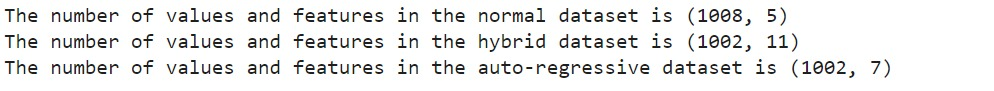
\includegraphics[width=0.9\linewidth]{fig11.jpeg}
		\caption{Table of Different Data sets.}\label{fig12}
	\end{figure}
	
	
	
	\begin{figure}[!ht]
		\centering
		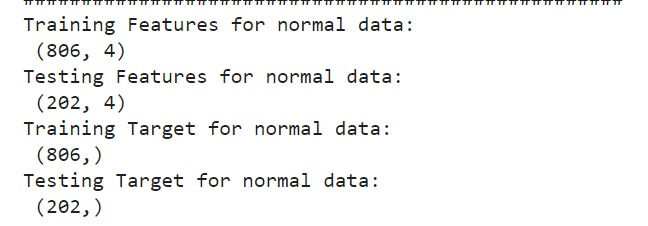
\includegraphics[width=0.6\linewidth]{nor.jpeg}
		\caption{Table of Normal Data set.}\label{fig13}
	\end{figure}
	
	\begin{figure}[!ht]
		\centering
		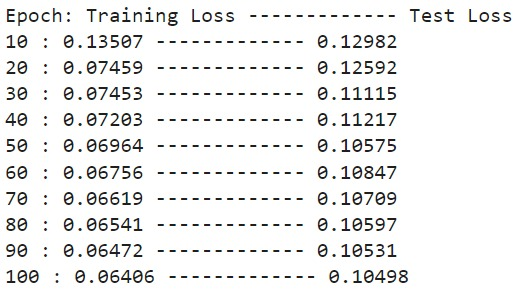
\includegraphics[width=0.5\linewidth]{enor.jpeg}
		\caption{Table of Train and test loss of the normal data over 100 epochs.}	\label{fig17}
	\end{figure}
	
	
	
	\begin{figure}[!ht]
		\centering
		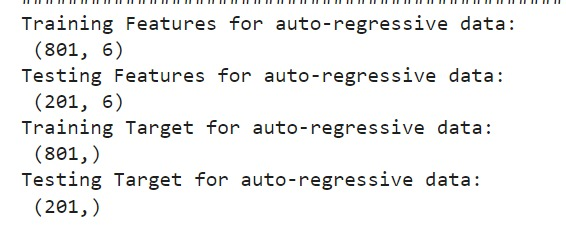
\includegraphics[width=0.5\linewidth]{auto.jpeg}
		\caption{Table of Auto-Regressive Data set.}	\label{fig14}
	\end{figure}
	
	\begin{figure}[!ht]
		\centering
		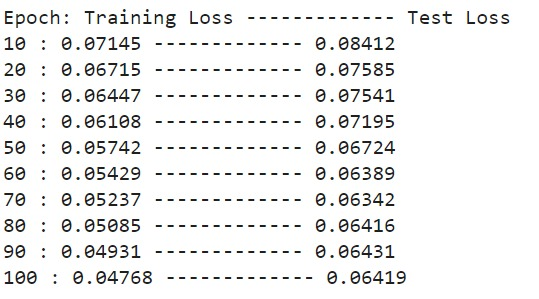
\includegraphics[width=0.5\linewidth]{eauto.jpeg}
		\caption{Table of Train and test loss of the auto regressive data over 100 epochs.}\label{fig18}
	\end{figure}
	
	
	
	
	\begin{figure}[!ht]
		\centering
		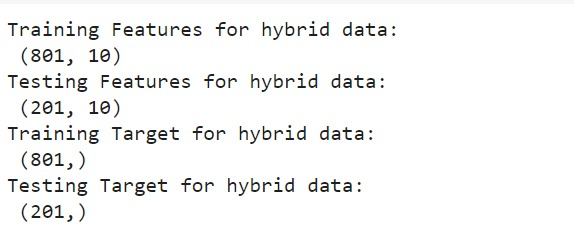
\includegraphics[width=0.6\linewidth]{hyb.jpeg}
		\caption{Table of Hybrid Data set.}	\label{fig15}
	\end{figure}
	
	We spilt all with 20 percent as testing data, and a random state = 42 as shown in fig. $\ref{fig13}$, $\ref{fig14}$, $\ref{fig15}$.\\
	The neural network is trained with two hidden layers consisting of 50 neurons each, a learning rate of 1e-2, 100 epochs, the ReLU activation function,  MSE as the error metric and the ADAM optimizer. Xavier Initialization for the weights and biases shown in Fig. $\ref{fig30}$.
	
	
	\begin{figure}[!ht]
		\centering
		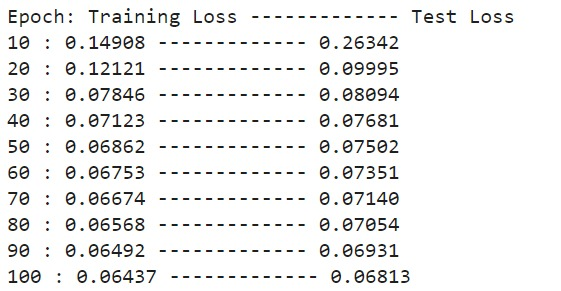
\includegraphics[width=0.5\linewidth]{Ehyb.jpeg}
		\caption{Table of Train loss and test loss of the hybrid data over 100 epochs.}\label{fig19}
	\end{figure}
	
	
	
	
	\begin{figure}[!ht]
		\centering
		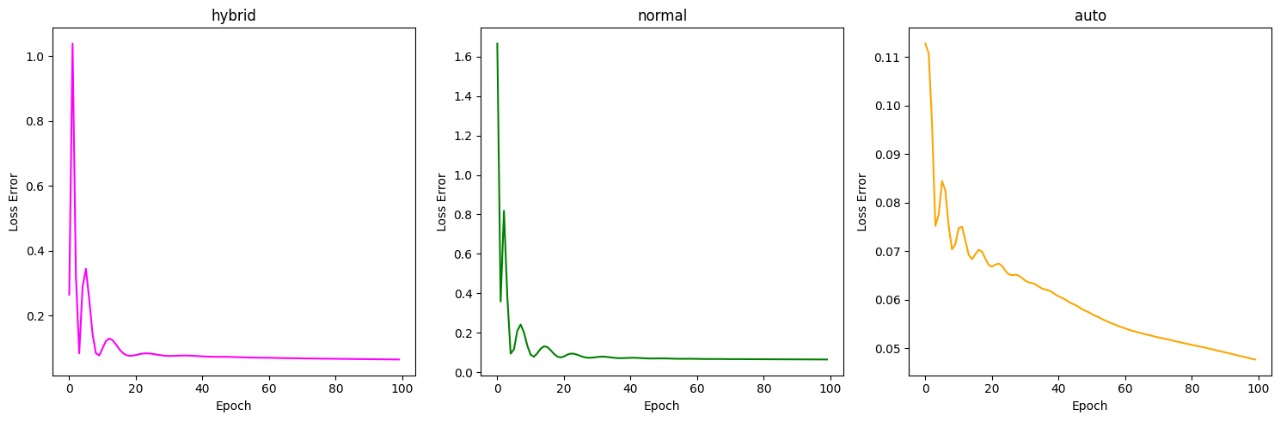
\includegraphics[width=0.9\linewidth]{fig12.jpeg}
		\caption{Comparison of the loss function plots of all three neural network models.}\label{fig20}
	\end{figure}
	
	
	\begin{figure}[!ht]
		\centering
		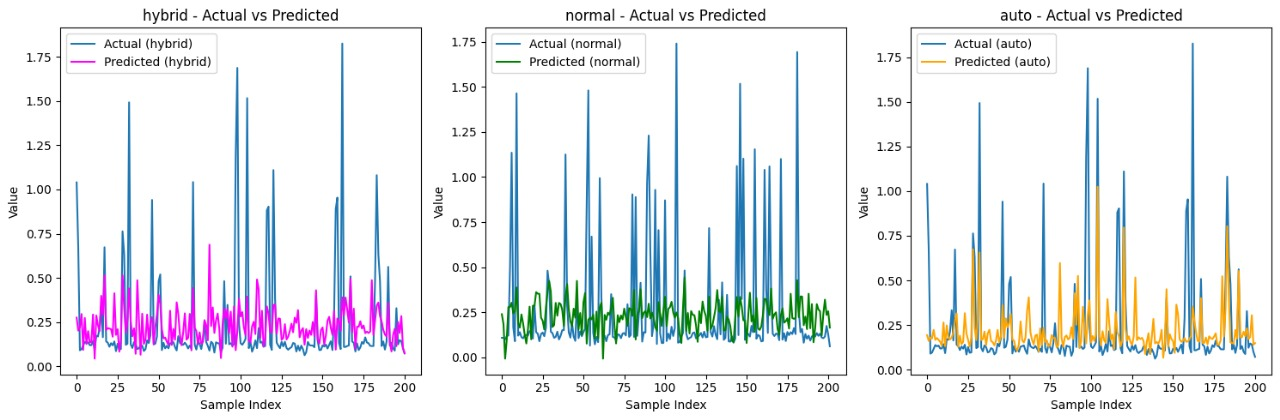
\includegraphics[width=0.9\linewidth]{fig17.jpeg}
		\caption{Plot of the actual test data vs predictions from all three neural network models.}\label{fig30}
	\end{figure}
	
	
	We now make a comparison based on the number of layers and neurons, using the neural network trained on the hybrid data shown in Fig.$\ref{fig21}$, $\ref{fig22}$.\\
	Here, we consider the train loss and test loss as we increase the number of layers from 2 to 8 and the number of neurons from 10 to 30. The table $\ref{fig17}$, $\ref{fig18}$ ,$\ref{fig19}$ below shows the values obtained after training for 100 epochs each. We can see that from the test loss table, the model showed a slight overfitting with large number of layers and neurons, as the test loss value is high compared to the train loss value.
	
	
	\begin{figure}[!ht]
		\centering
		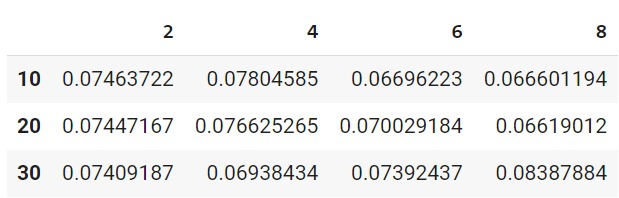
\includegraphics[width=0.7\linewidth]{fig13.jpeg}
		\label{fig21}
		\caption{Table shows the test loss comparison over different layers and neurons.}
	\end{figure}
	
	
	\begin{figure}[!ht]
		\centering
		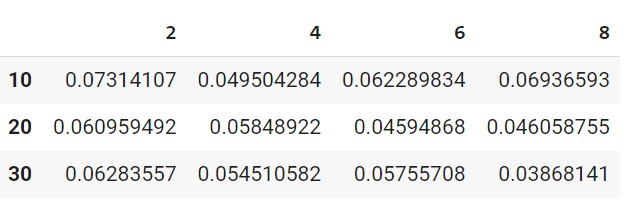
\includegraphics[width=0.7\linewidth]{fig14.jpeg}
		\label{fig22}
		\caption{Table shows the Train loss comparison over different layers and neurons.}
	\end{figure}
	
	
	Finally, we make a comparison based on different activation functions. We consider ReLU, Tanh, Tanhshrink, softsign, GeLU, CeLU and LeakyReLU in Fig.$\ref{fig23}$. \\
	For this final comparison, we consider two hidden layers with 10 neurons each.\\
	We provide a comparison based on the test loss and the train loss in Fig.$\ref{fig24}$..
	
	
	\begin{figure}[!ht]
		\centering
		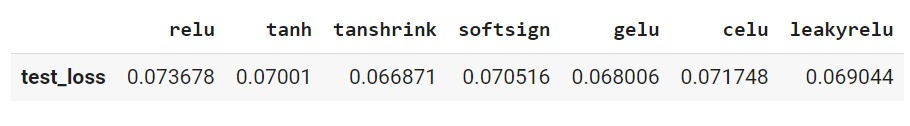
\includegraphics[width=0.8\linewidth]{fig15.jpeg}
		\caption{Table shows the test loss comparison with different activation functions. The Tanshrink activation function have the least test loss.}	\label{fig23}
	\end{figure}
	
	
	\begin{figure}[!ht]
		\centering
		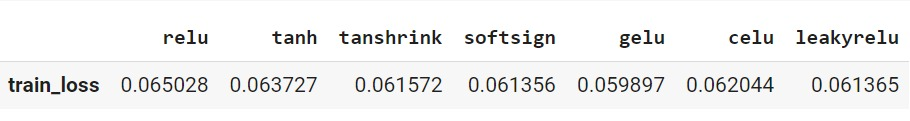
\includegraphics[width=0.8\linewidth]{fig16.jpeg}
		\caption{Table shows the train loss comparison between the activation functions.}\label{fig24}
	\end{figure}
	
	
	\subsubsection{Clustering}
	We preprocess the data using "StandardScaler" from Sklearn, and then perform the K-Means clustering on the preprocessed data with 3 clusters.  We first print the mean consumption for each cluster in Fig.$\ref{fig25}$.
	
	
	\begin{figure}[!ht]
		\centering
		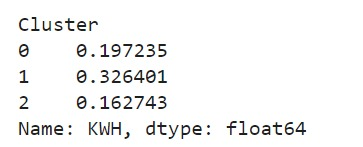
\includegraphics[width=0.5\linewidth]{fig18.jpeg}
		\caption{figure shows the mean consumption for each cluster.}\label{fig25}
	\end{figure}
	
	Then we check the cluster size. The first cluster contains 349 samples , the second contains 344 samples and the third contains 315 samples as shown on the 
	Fig.$\ref{fig26}$.
	
	
	
	\begin{figure}[!ht]
		\centering
		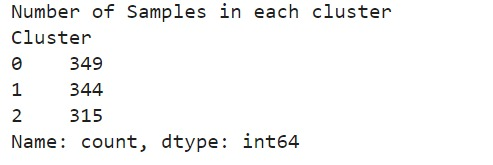
\includegraphics[width=0.5\linewidth]{fig19.jpeg}
		\caption{figure shows the cluster size.}\label{fig26}
	\end{figure}
	
	To visualize, since we have four the input features, we first reduce the dimensions using Principal Component Analysis (PCA) to two dimensions, then we plot the reduced features. We can see that two centroids seems very close to each other can be seen in Fig.$\ref{fig27}$.
	
	
	\begin{figure}[!ht]
		\centering
		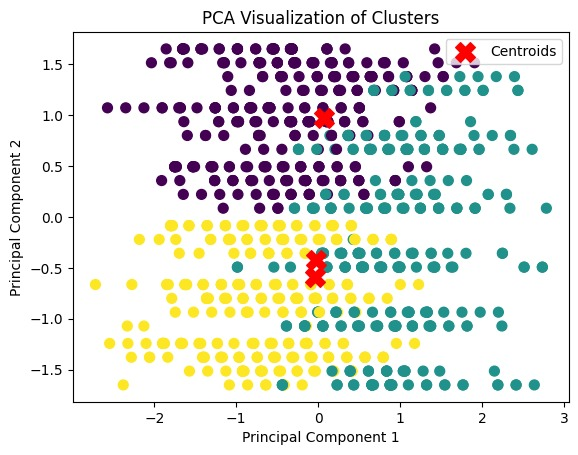
\includegraphics[width=0.5\linewidth]{fig20.jpeg}
		\caption{figure shows the reduced features.}\label{fig27}
	\end{figure}
	
	Due to this, we try to check for the optimal number of clusters using the Elbow method. We can see that the inertia plot against the number of clusters is almost a smooth curve. This implies that there may be no finite number of optimal clusters. There are many interpretations to this, which includes the presence of outliers shown in Fig.$\ref{fig28}$.
	
	
	\begin{figure}[!ht]
		\centering
		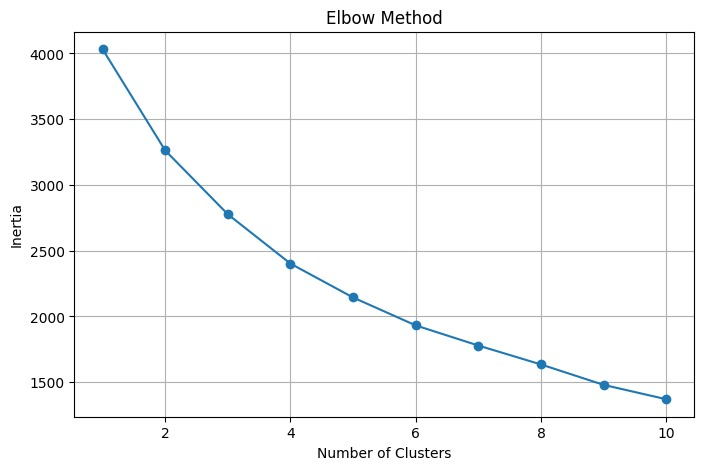
\includegraphics[width=0.5\linewidth]{fig21.jpeg}
		\caption{figure shows optimal number of clusters using the Elbow method.}\label{fig28}
	\end{figure}
	
	
	We also use the Silhouette Score method to verify the optimal number of clusters. However, this score continue to increase as the number of clusters increase, implying that we have similar issue as the elbow method. We conclude that the presence of outliers is a major factor for this can be visualize in Fig.$\ref{fig29}$.
	
	\begin{figure}[!ht]
		\centering
		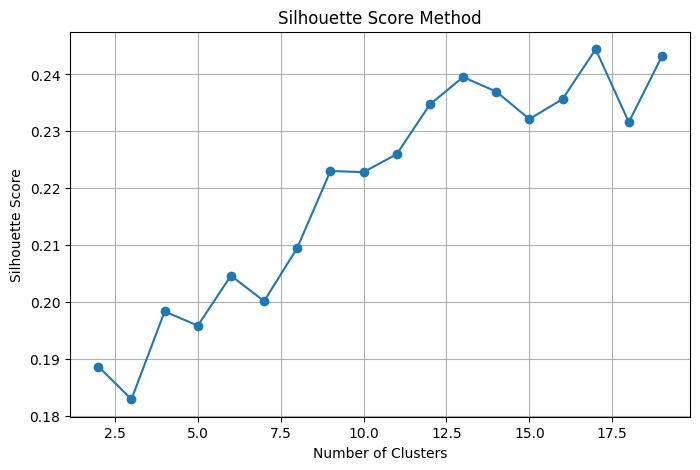
\includegraphics[width=0.5\linewidth]{fig22.jpeg}
		\caption{figure shows Silhouette Score method to verify the optimal number of clusters.}\label{fig29}
	\end{figure}
	
	\subsubsection{Forecasting}
	
	We analyze the household consumption, by forecasting for the next 100 periods using a neural network. Here, we train the whole Team 1 data set to forecast on the next 100 periods given in Fig.$\ref{fig32}$.
	
	\begin{figure}[!ht]
		\centering
		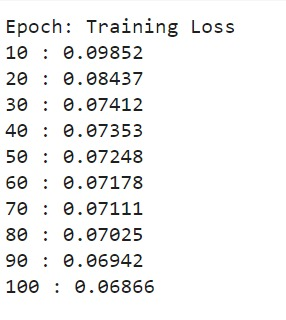
\includegraphics[width=0.25\linewidth]{fig23.jpeg}
		\caption{figure shows forecasting for the next 100 periods.}\label{fig32}
	\end{figure}
	
	
	The predictions(forecast) is shown in this  Fig.$\ref{fig33}$, and added to a csv file which we named $\text{\textbf{forecast}}$.
	
	\begin{figure}[!ht]
		\centering
		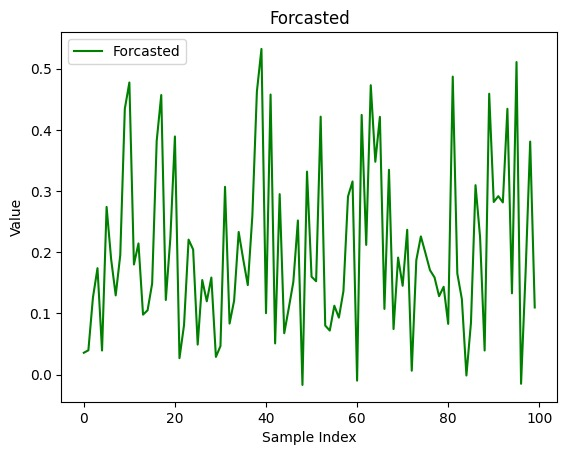
\includegraphics[width=0.4\linewidth]{fig24.jpeg}
		\caption{figure shows predictions(forecast).}\label{fig33}
	\end{figure}
	
	
	
	
	
	\clearpage
	%\phantomsection
	\addcontentsline{toc}{section}{Conclusion}
	
	%\newpage
	%
	%\section{Conclusion}
	\textbf{\Large {Conclusion}}\\
	\newline
	This report investigates optimal techniques for data fitting and forecasting using advanced analytical tools, including Exploratory Data Analysis (EDA), Variance-Covariance Analysis, Linear Regression, Singular Value Decomposition (SVD), Time Series Analysis, and Neural Networks. The study systematically assessed these techniques to address the challenges posed by energy consumption datasets characterized by non-normality, multicollinearity, and the presence of outliers.\\
	
	The findings highlight the robustness of hybrid models combining machine learning and statistical techniques. EDA provided key insights into data structure, outliers, and distribution, which were critical for preprocessing and feature selection. Variance-Covariance analysis underscored multicollinearity's impact, leading to targeted feature engineering. SVD successfully reduced dimensionality and noise, offering a computationally efficient baseline model. Time Series Analysis captured sequential dependencies and seasonality, while Neural Networks excelled in learning non-linear relationships with optimized architectures and activation functions. The study also evaluated neural network performance using multiple activation functions, highlighting the effectiveness of techniques like Tanhshrink and Softsign for specific data characteristics.\\
	
	Comparative analysis revealed that hybrid models integrating SVD and neural networks yielded superior accuracy and scalability. However, challenges such as overfitting with deep neural networks and loss of data during outlier treatment were noted, necessitating further refinement in these methods. This research contributes to understanding how different modeling approaches perform under varying data conditions and provides actionable insights for energy consumption forecasting.\\
	
	Future work could involve exploring ensemble techniques to combine the strengths of statistical and machine learning models further. These findings hold significant implications for real-world applications, such as optimizing energy usage, designing efficient appliances, and contributing to sustainable development initiatives.
	
	\clearpage
	%\phantomsection
	\addcontentsline{toc}{section}{References}
	
	
	% Generated by IEEEtran.bst, version: 1.14 (2015/08/26)
	\begin{thebibliography}{1}
		\providecommand{\url}[1]{#1}
		\csname url@samestyle\endcsname
		\providecommand{\newblock}{\relax}
		\providecommand{\bibinfo}[2]{#2}
		\providecommand{\BIBentrySTDinterwordspacing}{\spaceskip=0pt\relax}
		\providecommand{\BIBentryALTinterwordstretchfactor}{4}
		\providecommand{\BIBentryALTinterwordspacing}{\spaceskip=\fontdimen2\font plus
			\BIBentryALTinterwordstretchfactor\fontdimen3\font minus
			\fontdimen4\font\relax}
		\providecommand{\BIBforeignlanguage}[2]{{%
				\expandafter\ifx\csname l@#1\endcsname\relax
				\typeout{** WARNING: IEEEtran.bst: No hyphenation pattern has been}% 
				\typeout{** loaded for the language `#1'. Using the pattern for}% 
				\typeout{** the default language instead.}% 
				\else
				\language=\csname l@#1\endcsname
				\fi
				#2}}
		\providecommand{\BIBdecl}{\relax}
		\BIBdecl
		
		\bibitem{jt}
		J.~W. Tukey, \emph{Exploratory data analysis}.\hskip 1em plus 0.5em minus 0.4em\relax Reading/Addison-Wesley, 1977.
		
		\bibitem{jw}
		J.~Wichern et al., ``Using household survey data to identify large-scale food security patterns across Uganda,'' \emph{PLoS One}, vol.~13, no.~12, p.~e0208714, 2018.
		
		\bibitem{gvl}
		G.~H. Golub and C.~F. Van Loan, \emph{Matrix computations}.\hskip 1em plus 0.5em minus 0.4em\relax JHU Press, 2013.
		
		\bibitem{box}
		G.~E.~P. Box et al., \emph{Time series analysis: forecasting and control}.\hskip 1em plus 0.5em minus 0.4em\relax John Wiley \& Sons, 2015.
		
		\bibitem{gf}
		J.~Heaton, ``Ian goodfellow, yoshua bengio, and aaron courville: Deep learning: The mit press, 2016, 800 pp, isbn: 0262035618,'' \emph{Genetic programming and evolvable machines}, vol.~19, no.~1, pp.~305--307, 2018.
		
		
		\bibitem{slim} 
		Belhaiza, Slim, and Sara Al-Abdallah. "A Neural Network Forecasting Approach for the Smart Grid Demand Response Management Problem." Energies 17.10 (2024): 2329.
	\end{thebibliography}
	
	
	
	
	
	
	
\end{document}